\section{Biểu Diễn Trạng Thái}

\begin{frame}{Định nghĩa Không gian trạng thái}
  \begin{columns}[T,totalwidth=\textwidth]
    \begin{column}{0.48\textwidth}
      \[
        S=\langle B,p,c_h,h\rangle
      \]
      \begin{itemize}[<+->]
        \item $B$: bàn cờ $10 \times 9$.
        \item $p$: bên đi.
        \item $c_h$: bộ đếm luật 60 nước.
        \item $h$: lịch sử để undo và phát hiện lặp.
      \end{itemize}
    \end{column}
    \begin{column}{0.48\textwidth}
      \centering
      \begin{figure}
        \begin{tikzpicture}[node distance=0.45cm]
          \node[redbox, text width=1.55cm] (b) {$B$\\Board};
          \onslide<2->\node[darkbox, text width=1.55cm, below=0.25cm of b] (p) {$p$\\Side};
          \onslide<3->\node[darkbox, text width=1.55cm, below=0.25cm of p] (c) {$c_h$\\Clock};
          \onslide<4->\node[darkbox, text width=1.55cm, below=0.25cm of c] (h) {$h$\\History};
          \onslide<1->\node[fit=(b)(p)(c)(h), draw=hustred, rounded corners=2pt, inner sep=0.18cm] {};
        \end{tikzpicture}
        \caption{Không gian trạng thái}
      \end{figure}
    \end{column}
  \end{columns}
\end{frame}

\begin{frame}{Biểu diễn $B$ bằng Bitboard \code{u128}}
  \begin{columns}[T,totalwidth=\textwidth]
    \begin{column}{0.42\textwidth}
      \begin{itemize}[<+->]
        \item Cờ tướng có 90 ô nên \code{u64} không đủ.
        \item Lingine dùng \code{u128}; 90 bit đầu biểu diễn 90 ô.
        \item Bitboard theo màu và theo loại quân giúp query nhanh.
        \item Có thể tìm chỉ số của những bit bật bằng instruction TZCNT của x86\_64 chỉ tốn vài chu kỳ CPU.
      \end{itemize}
    \end{column}
    \begin{column}{0.54\textwidth}
      \centering
        \begin{figure}[H]
    \centering
    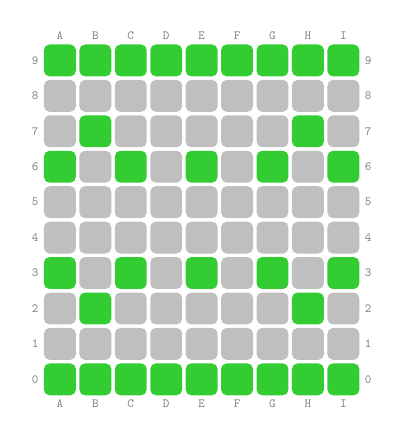
\begin{tikzpicture}[
        font=\ttfamily,
        scale=0.45,
        transform shape,
        blank square/.style={fill=gray!50, rounded corners=2pt, minimum size=0.9cm, thick},
        active square/.style={fill=green!60!gray, rounded corners=2pt, minimum size=0.9cm, thick},
    ]

    % Định nghĩa chuỗi bitboard phẳng gồm đúng 90 phần tử (từ ô A9 đến I0)
    \def\bitboarddata{
        1,1,1,1,1,1,1,1,1, % Hàng 9
        0,0,0,0,0,0,0,0,0, % Hàng 8
        0,1,0,0,0,0,0,1,0, % Hàng 7
        1,0,1,0,1,0,1,0,1, % Hàng 6
        0,0,0,0,0,0,0,0,0, % Hàng 5
        0,0,0,0,0,0,0,0,0, % Hàng 4
        1,0,1,0,1,0,1,0,1, % Hàng 3
        0,1,0,0,0,0,0,1,0, % Hàng 2
        0,0,0,0,0,0,0,0,0, % Hàng 1
        1,1,1,1,1,1,1,1,1  % Hàng 0
    }

    % Duyệt qua 90 phần tử
    \foreach \bit [count=\idx from 0] in \bitboarddata {
        % Tọa độ X (Cột): từ 0 đến 8
        \pgfmathtruncatemacro{\realX}{mod(\idx, 9)}
        % Tọa độ Y (Hàng): Sử dụng floor để cố định chính xác chỉ số hàng không bị làm tròn sai
        \pgfmathtruncatemacro{\realY}{9 - floor(\idx / 9)}
        
        % Chọn kiểu hiển thị dựa trên giá trị bit
        \def\squarestyle{blank square}
        \ifnum\bit=1
            \def\squarestyle{active square}
        \fi
        
        % Vẽ ô vuông
        \node[\squarestyle] (sq-\realX-\realY) at (\realX, \realY) {};
    }

    % Vẽ nhãn số cho các Hàng (0 -> 9) ở hai bên lề
    \foreach \y in {0,...,9} {
        \node[text=gray] at (-0.7, \y) {\y};
        \node[text=gray] at (8.7, \y) {\y};
    }

    % Vẽ nhãn chữ cho các Cột (A -> I) ở trên và dưới
    \foreach \x/\letter in {0/A, 1/B, 2/C, 3/D, 4/E, 5/F, 6/G, 7/H, 8/I} {
        \node[text=gray] at (\x, 9.7) {\letter};
        \node[text=gray] at (\x, -0.7) {\letter};
    }

    \end{tikzpicture}
    \caption{Bitboard cho Bàn cờ tướng bắt đầu}
    \label{fig:xiangqi_bitboard}
\end{figure}
    \end{column}
  \end{columns}
\end{frame}

\begin{frame}{Ví dụ truy vấn tìm kiếm quân xe đỏ}
  \vspace{-0.5cm}
  \centering
  \begin{columns}[T,totalwidth=\textwidth]
    \begin{column}{0.25\textwidth}
      \centering
        \begin{figure}[H]
    \centering
    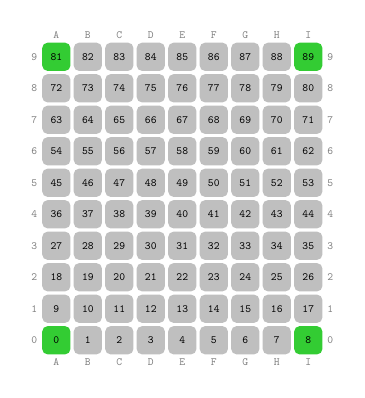
\begin{tikzpicture}[
        font=\ttfamily,
        scale=0.4,
        transform shape,
        blank square/.style={fill=gray!50, rounded corners=2pt, minimum size=0.9cm, thick},
        active square/.style={fill=green!60!gray, rounded corners=2pt, minimum size=0.9cm, thick},
    ]

    % Định nghĩa chuỗi bitboard phẳng gồm đúng 90 phần tử (từ ô A9 đến I0)
    \def\bitboarddata{
        1,0,0,0,0,0,0,0,1, % Hàng 9
        0,0,0,0,0,0,0,0,0, % Hàng 8
        0,0,0,0,0,0,0,0,0, % Hàng 7
        0,0,0,0,0,0,0,0,0, % Hàng 6
        0,0,0,0,0,0,0,0,0, % Hàng 5
        0,0,0,0,0,0,0,0,0, % Hàng 4
        0,0,0,0,0,0,0,0,0, % Hàng 3
        0,0,0,0,0,0,0,0,0, % Hàng 2
        0,0,0,0,0,0,0,0,0, % Hàng 1
        1,0,0,0,0,0,0,0,1  % Hàng 0
    }

    % Duyệt qua 90 phần tử
    \foreach \bit [count=\idx from 0] in \bitboarddata {
        % Tọa độ X (Cột): từ 0 đến 8
        \pgfmathtruncatemacro{\realX}{mod(\idx, 9)}
        % Tọa độ Y (Hàng): Sử dụng floor để cố định chính xác chỉ số hàng không bị làm tròn sai
        \pgfmathtruncatemacro{\realY}{9 - floor(\idx / 9)}
        
        % Chọn kiểu hiển thị dựa trên giá trị bit
        \def\squarestyle{blank square}
        \ifnum\bit=1
            \def\squarestyle{active square}
        \fi
        
        % Vẽ ô vuông
          \pgfmathtruncatemacro{\bitposition}{\realY * 9 + \realX}
          % Vẽ ô vuông
          \node[\squarestyle] (sq-\realX-\realY) at (\realX, \realY) {\bitposition};
    }

    % Vẽ nhãn số cho các Hàng (0 -> 9) ở hai bên lề
    \foreach \y in {0,...,9} {
        \node[text=gray] at (-0.7, \y) {\y};
        \node[text=gray] at (8.7, \y) {\y};
    }

    % Vẽ nhãn chữ cho các Cột (A -> I) ở trên và dưới
    \foreach \x/\letter in {0/A, 1/B, 2/C, 3/D, 4/E, 5/F, 6/G, 7/H, 8/I} {
        \node[text=gray] at (\x, 9.7) {\letter};
        \node[text=gray] at (\x, -0.7) {\letter};
    }

    \end{tikzpicture}
    \caption*{Bitboard cho các quân xe}
\end{figure}
    \end{column}
    \pause
    \begin{column}{0.1\textwidth}
      \centering
      \vspace{6em}
      \hspace{1em}\Huge $\&$
    \end{column}
    \pause 
    \begin{column}{0.25\textwidth}
        \centering
          \begin{figure}[H]
      \centering
      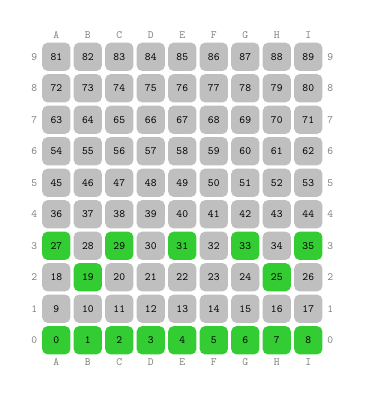
\begin{tikzpicture}[
          font=\ttfamily,
          scale=0.4,
          transform shape,
          blank square/.style={fill=gray!50, rounded corners=2pt, minimum size=0.9cm, thick},
          active square/.style={fill=green!60!gray, rounded corners=2pt, minimum size=0.9cm, thick},
      ]

      % Định nghĩa chuỗi bitboard phẳng gồm đúng 90 phần tử (từ ô A9 đến I0)
      \def\bitboarddata{
          0,0,0,0,0,0,0,0,0, % Hàng 9
          0,0,0,0,0,0,0,0,0, % Hàng 8
          0,0,0,0,0,0,0,0,0, % Hàng 7
          0,0,0,0,0,0,0,0,0, % Hàng 6
          0,0,0,0,0,0,0,0,0, % Hàng 5
          0,0,0,0,0,0,0,0,0, % Hàng 4
          1,0,1,0,1,0,1,0,1, % Hàng 3
          0,1,0,0,0,0,0,1,0, % Hàng 2
          0,0,0,0,0,0,0,0,0, % Hàng 1
          1,1,1,1,1,1,1,1,1  % Hàng 0
      }

      % Duyệt qua 90 phần tử
      \foreach \bit [count=\idx from 0] in \bitboarddata {
          % Tọa độ X (Cột): từ 0 đến 8
          \pgfmathtruncatemacro{\realX}{mod(\idx, 9)}
          % Tọa độ Y (Hàng): Sử dụng floor để cố định chính xác chỉ số hàng không bị làm tròn sai
          \pgfmathtruncatemacro{\realY}{9 - floor(\idx / 9)}
          
          % Chọn kiểu hiển thị dựa trên giá trị bit
          \def\squarestyle{blank square}
          \ifnum\bit=1
              \def\squarestyle{active square}
          \fi
          
          \pgfmathtruncatemacro{\bitposition}{\realY * 9 + \realX}
          % Vẽ ô vuông
          \node[\squarestyle] (sq-\realX-\realY) at (\realX, \realY) {\bitposition};
      }

      % Vẽ nhãn số cho các Hàng (0 -> 9) ở hai bên lề
      \foreach \y in {0,...,9} {
          \node[text=gray] at (-0.7, \y) {\y};
          \node[text=gray] at (8.7, \y) {\y};
      }

      % Vẽ nhãn chữ cho các Cột (A -> I) ở trên và dưới
      \foreach \x/\letter in {0/A, 1/B, 2/C, 3/D, 4/E, 5/F, 6/G, 7/H, 8/I} {
          \node[text=gray] at (\x, 9.7) {\letter};
          \node[text=gray] at (\x, -0.7) {\letter};
      }

      \end{tikzpicture}
      \caption*{Bitboard cho các quân bên đỏ}
    \end{figure}
    \end{column}
    \pause
    \begin{column}{0.1\textwidth}
      \centering
      \vspace{6.5em}
      \hspace{1em}\Huge $=$
    \end{column}
    \pause
    \begin{column}{0.25\textwidth}
      \centering
        \begin{figure}[H]
    \centering
    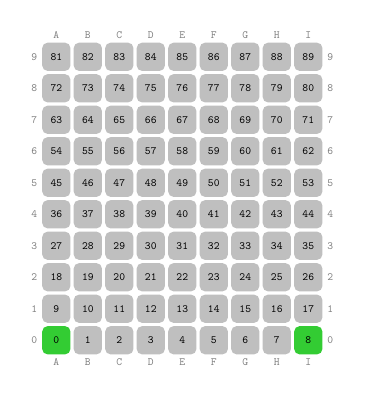
\begin{tikzpicture}[
        font=\ttfamily,
        scale=0.4,
        transform shape,
        blank square/.style={fill=gray!50, rounded corners=2pt, minimum size=0.9cm, thick},
        active square/.style={fill=green!60!gray, rounded corners=2pt, minimum size=0.9cm, thick},
    ]

    % Định nghĩa chuỗi bitboard phẳng gồm đúng 90 phần tử (từ ô A9 đến I0)
    \def\bitboarddata{
        0,0,0,0,0,0,0,0,0, % Hàng 9
        0,0,0,0,0,0,0,0,0, % Hàng 8
        0,0,0,0,0,0,0,0,0, % Hàng 7
        0,0,0,0,0,0,0,0,0, % Hàng 6
        0,0,0,0,0,0,0,0,0, % Hàng 5
        0,0,0,0,0,0,0,0,0, % Hàng 4
        0,0,0,0,0,0,0,0,0, % Hàng 3
        0,0,0,0,0,0,0,0,0, % Hàng 2
        0,0,0,0,0,0,0,0,0, % Hàng 0
        1,0,0,0,0,0,0,0,1  % Hàng 1
    }

    % Duyệt qua 90 phần tử
    \foreach \bit [count=\idx from 0] in \bitboarddata {
        % Tọa độ X (Cột): từ 0 đến 8
        \pgfmathtruncatemacro{\realX}{mod(\idx, 9)}
        % Tọa độ Y (Hàng): Sử dụng floor để cố định chính xác chỉ số hàng không bị làm tròn sai
        \pgfmathtruncatemacro{\realY}{9 - floor(\idx / 9)}
        
        % Chọn kiểu hiển thị dựa trên giá trị bit
        \def\squarestyle{blank square}
        \ifnum\bit=1
            \def\squarestyle{active square}
        \fi
        
        % Vẽ ô vuông
          \pgfmathtruncatemacro{\bitposition}{\realY * 9 + \realX}
          % Vẽ ô vuông
          \node[\squarestyle] (sq-\realX-\realY) at (\realX, \realY) {\bitposition};
    }

    % Vẽ nhãn số cho các Hàng (0 -> 9) ở hai bên lề
    \foreach \y in {0,...,9} {
        \node[text=gray] at (-0.7, \y) {\y};
        \node[text=gray] at (8.7, \y) {\y};
    }

    % Vẽ nhãn chữ cho các Cột (A -> I) ở trên và dưới
    \foreach \x/\letter in {0/A, 1/B, 2/C, 3/D, 4/E, 5/F, 6/G, 7/H, 8/I} {
        \node[text=gray] at (\x, 9.7) {\letter};
        \node[text=gray] at (\x, -0.7) {\letter};
    }

    \end{tikzpicture}
    \caption*{Bitboard cho các quân xe bên đỏ}
\end{figure}
    \end{column}
  \end{columns}

\end{frame}

\begin{frame}{Nén nước đi 16-bit}
  \centering
  \begin{figure}[H]
    \centering
    \begin{tikzpicture}[font=\sffamily, scale=0.8, transform shape]
        % Draw 16 bit boxes
        \foreach \i in {0,...,6} \node[draw, minimum width=0.8cm, minimum height=0.8cm, anchor=south west, fill=blue!20] (bit\i) at (\i*0.8, 0) {\i};
        \foreach \i in {7,...,13} \node[draw, minimum width=0.8cm, minimum height=0.8cm, anchor=south west, fill=green!20] (bit\i) at (\i*0.8, 0) {\i};
        \foreach \i in {14,...,15} \node[draw, minimum width=0.8cm, minimum height=0.8cm, anchor=south west, fill=gray!20] (bit\i) at (\i*0.8, 0) {\i};
        
        % Labels above
        \draw[thick, decorate, decoration={brace, amplitude=5pt, raise=2pt}] 
            (bit0.north west) -- (bit6.north east) node[midway, above=8pt] {Ô đích (To) [0-6]};
            
        \draw[thick, decorate, decoration={brace, amplitude=5pt, raise=2pt}] 
            (bit7.north west) -- (bit13.north east) node[midway, above=8pt] {Ô nguồn (From) [7-13]};
            
        \draw[thick, decorate, decoration={brace, amplitude=5pt, raise=2pt}] 
            (bit14.north west) -- (bit15.north east) node[midway, above=8pt] {Trống [14-15]};
    \end{tikzpicture}
    \caption{Sơ đồ khối bit-field minh họa dữ liệu nước đi 16-bit trong Lingine}
    \label{fig:move_16bit_diagram}
\end{figure}
  \vspace{1em}
  \begin{itemize}[<+->]
    \item Kiểu \code{Move} là \code{NonZeroU16}.
    \item Nhỏ, truyền theo value, hợp cache.
    \item Phù hợp khi search cần duyệt hàng triệu nước đi.
  \end{itemize}
\end{frame}

\begin{frame}{Định danh trạng thái bằng Zobrist hashing}
  \begin{columns}[T,totalwidth=\textwidth]
    \begin{column}{0.48\textwidth} 
      \[ \text{Hash}(S_0) = Z_{side} \oplus \left( \bigoplus_{sq=0}^{89} Z_{piece(sq), sq} \right) \]
      Trong đó:
    \begin{itemize}
        \item $Z_{side}$ là $0$ nếu $side$ là Đỏ, ngược lại là một giá trị ngẫu nhiên.
        \item $Z_{piece(sq), sq}$ là giá trị ngẫu nhiên ứng với quân cờ đang ở ô $sq$. Nếu ô $sq$ trống thì giá trị này bằng $0$.
    \end{itemize}

    \end{column}
    \begin{column}{0.48\textwidth}

\begin{figure}[htbp]
  \vspace{-0.5cm}
    \centering
    \begin{tikzpicture}[
        scale=0.5,
        transform shape,
        font=\small,
        % Định nghĩa phong cách cho các khối lưu trình
        startstop/.style={rectangle, draw, fill=blue!10, minimum width=3.5cm, minimum height=0.7cm, rounded corners, thick, align=center},
        process/.style={rectangle, draw, fill=orange!15, minimum width=5.2cm, minimum height=0.7cm, thick, align=center},
        decision/.style={diamond, draw, fill=yellow!15, minimum width=3.2cm, minimum height=1cm, aspect=2, thick, align=center, inner sep=0pt},
        arrow/.style={-Latex}
    ]

    % --- KHỞI TẠO CÁC KHỐI THEO LUỒNG DỌC ---
    % Trạng thái băm ban đầu
    \node[startstop] (start) {Mã băm ban đầu: $hash$};
    
    \pause
    % Bước 1: Xóa quân ở ô đi
    \node[process, below=0.5cm of start] (xor1) {$hash \leftarrow hash \oplus Z[\text{piece}][\text{from}]$\\ (Xóa quân ở ô xuất phát)};

    % --- VẼ ĐƯỜNG NỐI LUỒNG DỮ LIỆU ---
    \draw[arrow] (start) -- (xor1);
    
    \pause
    % Bước 2: Đặt quân vào ô đến
    \node[process, below=0.5cm of xor1] (xor2) {$hash \leftarrow hash \oplus Z[\text{piece}][\text{to}]$\\ (Đặt quân vào ô đích)};
    \draw[arrow] (xor1) -- (xor2);
    
    \pause
    % Bước 3: Kiểm tra điều kiện ăn quân (Khối hình thoi)
    \node[decision, below=0.6cm of xor2] (check) {Có quân bị bắt\\ tại ô đích?};

    \draw[arrow] (xor2) -- (check);
    
    \pause
    % Bước 4: Nhánh YES - Loại bỏ quân bị ăn khỏi mã băm
    \node[process, below right=0.5cm and 4cm of check, anchor=north] (xor3) {$hash \leftarrow hash \oplus Z[\text{captured}][\text{to}]$\\ (Xóa quân bị ăn khỏi bàn cờ)};
    
    % Nhánh xử lý điều kiện Có/Không
    \draw[arrow] (check) -| node[above, pos=0.25] {Có (Yes)} (xor3);

    \pause
    % Bước 5: Đổi lượt đi (Điểm hội tụ của luồng điều kiện)
    \node[process, below=2.3cm of check] (xor4) {$hash \leftarrow hash \oplus Z_{\text{side}}$\\ (Thay đổi lượt đi)};

    \draw[arrow] (xor3) |- (xor4);
    \draw[arrow] (check) -- node[left] {Không (No)} (xor4);
    
    \pause
    % Trạng thái băm cuối cùng
    \node[startstop, fill=green!15, below=0.5cm of xor4] (end) {Mã băm mới: $hash'$};

    
    
    \draw[arrow] (xor4) -- (end);

    \end{tikzpicture}
    \caption{Sơ đồ luồng cập nhật vi phân Zobrist Hash sử dụng toán tử logic $\oplus$}
    \label{fig:zobrist_math_flow}
\end{figure}
      \centering
    \end{column}
  \end{columns}
\end{frame}

\begin{frame}{Bảng chuyển vị}
  \vspace{-1cm}
  \begin{figure}[htbp]
    \centering
    \begin{tikzpicture}[
        % Định nghĩa biến độ rộng cho 1 byte (ví dụ: 1 byte = 0.9cm)
        /tikz/byte width/.initial=1.4cm,
        % Định nghĩa phong cách chung cho các khối dữ liệu
        entry/.style={draw, minimum height=0.9cm, font=\ttfamily, align=center, thick},
        node distance=0cm,
        scale=0.62,
        transform shape
    ]
        % Đọc giá trị biến byte width vào macro \bw để dễ tính toán
        \pgfkeysgetvalue{/tikz/byte width}{\bw}

        % --- VẼ CÁC KHỐI DỮ LIỆU ---
        % Key: 8 bytes
        \node[entry, fill=blue!15, minimum width=8*\bw, anchor=south west] (key) at (0, 0) {key};
        % --- NHÃN SỐ BYTES PHÍA TRÊN ---
        \draw[thick, decorate, decoration={brace, amplitude=5pt, raise=2pt}] 
            (key.north west) -- (key.north east) node[midway, above=8pt] {\large 8 bytes};
          \pause
        
        % Score: 4 bytes
        \node[entry, fill=green!15, minimum width=4*\bw, anchor=south west] (score) at (key.south east) {score};
        \draw[thick, decorate, decoration={brace, amplitude=5pt, raise=2pt}] 
            (score.north west) -- (score.north east) node[midway, above=8pt] {\large 4 bytes};
          \pause
        
        % Move: 2 bytes
        \node[entry, fill=orange!15, minimum width=2*\bw, anchor=south west] (move) at (score.south east) {move};
        \draw[thick, decorate, decoration={brace, amplitude=5pt, raise=2pt}] 
            (move.north west) -- (move.north east) node[midway, above=8pt] {\large 2 bytes};
          \pause
        
        % Flags: 1 byte
        \node[entry, fill=red!15, minimum width=1*\bw, anchor=south west] (flags) at (move.south east) {flags};
        \draw[thick, decorate, decoration={brace, amplitude=4pt, raise=2pt}] 
            (flags.north west) -- (flags.north east) node[midway, above=8pt] {\large 1 byte};
          \pause
        
        % Depth: 1 byte
        \node[entry, fill=purple!15, minimum width=1*\bw, anchor=south west] (depth) at (flags.south east) {depth};

        \draw[thick, decorate, decoration={brace, amplitude=4pt, raise=2pt}] 
            (depth.north west) -- (depth.north east) node[midway, above=8pt] {\large 1 byte};

        % --- TỔNG KÍCH THƯỚC PHÍA DƯỚI ---
        \draw[thick, decorate, decoration={brace, mirror, amplitude=8pt, raise=5pt}] 
            (key.south west) -- (depth.south east) node[midway, below=0.5cm] {\large Tổng kích thước: 16 bytes};
            
    \end{tikzpicture}
    \caption{Sơ đồ phân bổ bộ nhớ của một entry Bảng chuyển vị trong Lingine}
    \label{fig:tt_storage_modified}

\end{figure}

\onslide<6->{Do tổng một entry là 16 bytes nên align tốt với cache, giúp tăng tốc độ truy vấn và tiết kiệm bộ nhớ.}
\end{frame}



